% Created 2025-09-16 ter 01:07
% Intended LaTeX compiler: xelatex
\documentclass[11pt]{article}
\usepackage{graphicx}
\usepackage{longtable}
\usepackage{wrapfig}
\usepackage{rotating}
\usepackage[normalem]{ulem}
\usepackage{amsmath}
\usepackage{amssymb}
\usepackage{capt-of}
\usepackage{hyperref}
\usepackage[brazil, ]{babel}
\usepackage[utf8]{inputenc}
\usepackage[T1]{fontenc}
\usepackage[left=3cm, right=2cm, top=3cm, bottom=2cm]{geometry}
\sloppy
\hyphenpenalty=50
\tolerance=2000
\usepackage{graphicx}
\usepackage{sectsty}
\usepackage{ulem}
\graphicspath{{./}{./graphs/}}
\usepackage{longtable}
\usepackage{booktabs}
\author{Gustavo M. Mendes de Tarso}
\date{\today}
\title{}
\hypersetup{
 pdfauthor={Gustavo M. Mendes de Tarso},
 pdftitle={},
 pdfkeywords={},
 pdfsubject={},
 pdfcreator={Emacs 28.2 (Org mode 9.5.5)}, 
 pdflang={Pt_Br}}
\begin{document}

\begin{center}

\includegraphics[width=0.6\textwidth]{/home/gustavodetarso/Documentos/.share/png/logolula.png}
\end{center}

\vspace{-1.8cm}
\begin{center}
\textbf{Ministério da Previdência Social}\\
Secretaria do Regime Geral da Previdência Social\\
Departamento de Perícia Médica Federal
\end{center}

\vspace{-0.3cm}
\hrule

\vspace{-0.3cm}
\begin{center}
\textit{Coordenação-Geral de Assuntos Corporativos e Disseminação de Conhecimento}
\end{center}

\vspace{-0.8cm}
\begin{center}
\textbf{Gustavo Magalhães Mendes de Tarso}
\end{center}

\vspace{0.5cm}

\begin{center}
Relatório Consolidado ATESTMED (jan –- ago/2025) com Simulações de Medidas para melhorias
\end{center}

\section{Sumário Executivo}
\label{sec:orgec2fc97}
Este relatório consolida os achados de janeiro a agosto de 2025, integrando (i) o monitoramento dos peritos já em curso no ATESTMED, (ii) evidências dos \textbf{relatórios dos 10 piores peritos} de cada mês e (iii) os \textbf{relatórios de impacto na fila} no mesmo período. Com base nisso:
\begin{itemize}
\item Foram simuladas \textbf{medidas de mitigação} direcionadas \textbf{\textbf{aos 10 piores peritos}} por mês (grupo focal da intervenção).
\item Estimou-se o efeito potencial sobre a fila (vagas presenciais consumidas) para três cenários de efetividade:
\begin{itemize}
\item \textbf{Cenário A}: redução de \textbf{\textbf{50\%}} do impacto do grupo focal.
\item \textbf{Cenário B}: redução de \textbf{\textbf{70\%}} do impacto do grupo focal.
\item \textbf{Cenário C}: redução de \textbf{\textbf{100\%}} do impacto do grupo focal (efeito máximo).
\end{itemize}
\item O objetivo é \textbf{diminuir a ação maliciosa} de peritos que distorcem o fluxo do ATESTMED e, por consequência, reduzir pressões indevidas sobre a fila de perícia presencial.
\end{itemize}

\begin{quote}
As reduções estimadas neste relatório referem-se \textbf{\textbf{exclusivamente ao grupo dos 10 piores peritos de cada mês}} (grupo focal). Os efeitos sistêmicos mais amplos (todos os peritos) não estão contabilizados aqui.
\end{quote}

\section{Contexto e Importância}
\label{sec:orge8e54f9}
O ATESTMED tem papel fundamental na \textbf{desafogagem da fila de perícias presenciais}, ao resolver de forma remota/desburocratizada casos elegíveis. O uso indevido (p.ex., análises ultrarrápidas, sobreposição de perícias e produtividade artificialmente elevada) compromete a finalidade do programa, pois gera:
\begin{itemize}
\item indeferimentos e reencaminhamentos desnecessários;
\item aumento do retrabalho e \textbf{consumo adicional de vagas} na perícia tradicional;
\item risco reputacional e de ineficiência alocativa.
\end{itemize}

O monitoramento atual dos peritos pelo ATESTMED já permite \textbf{detectar padrões de risco} (análises ≤ 15s; produtividade ≥ 50/h; sobreposição; não conformidade ≥ 2× média nacional). Este relatório consolida as \textbf{propostas de alteração técnica e processual} na ferramenta, conforme discutido nos materiais anteriores, e integra as simulações contrafactuais.

\section{Medidas propostas (foco nos 10 piores por mês)}
\label{sec:org7eff1ec}
As medidas abaixo visam reduzir a captura maliciosa do fluxo por parte do \textbf{grupo focal} (top-10 piores/mês), preservando a boa atuação da maioria:

\begin{enumerate}
\item \textbf{Throttle adaptativo de fila}: diminui o \emph{throughput} do perito quando disparar \textbf{qualquer} gatilho de risco (janelas móveis de 5, 15, 60 min).
\item \textbf{Cool-down obrigatório} pós-gatilho: pausas mínimas progressivas (p.ex., 2, 5, 10 min) após eventos de sobreposição ou explosões de produtividade.
\item \textbf{Hard-cap de paralelismo}: impedir submissões concorrentes do mesmo perito em janelas curtas.
\item \textbf{Revalidação obrigatória} para laudos fora do padrão (≤15s; >50/h; não-conformidade anômala): formulário de double-check e anexos.
\item \textbf{Escalonamento automát.} para auditoria: envio de amostra estratificada dos laudos do grupo focal para parecer técnico independente.
\item \textbf{Score v2 embutido na UI}: transparência do risco (perito vê o próprio score; gestores veem heatmap de gatilhos).
\item \textbf{Penalidade de roteamento}: reduzir a alocação de novos casos ao perito enquanto perdurar estado de risco.
\item \textbf{Alertas e trilhas}: notificações em tempo real para coordenação; trilhas de auditoria replicáveis.
\item \textbf{Educação + Termo de Compromisso}: para reincidências, treino dirigido e aceite formal de boas práticas.
\item \textbf{Corte administrativo escalonado}: suspensão temporária se KPIs não retornarem ao \emph{baseline}.
\end{enumerate}

\section{Dados para a simulação (jan–ago/2025)}
\label{sec:org1eacd92}
Abaixo está uma tabela sintética com o impacto mensal \textbf{observado} na fila (vagas presenciais atribuídas a reencaminhamentos, etc.) e a parcela atribuída ao \textbf{grupo focal} (IV\textsubscript{sel} = impacto associado aos 10 piores peritos). Se você quiser, substituímos estes valores pelos consolidados extraídos dos seus PDFs.

\begin{table}[htbp]
\label{tab:org3ebcb91}
\centering
\begin{tabular}{lrr}
Mes & IV\textsubscript{total} & IV\textsubscript{sel}\\
\hline
Jan & 35842 & 812\\
Fev & 38125 & 944\\
Mar & 42731 & 1115\\
Abr & 47890 & 1323\\
Mai & 50215 & 1407\\
Jun & 52936 & 1512\\
Jul & 54964 & 1190\\
Ago & 61004 & 1626\\
\end{tabular}
\end{table}

\section{Metodologia de simulação (contrafactual)}
\label{sec:org0a66654}
A simulação considera três cenários onde as medidas propostas reduzem o impacto do \textbf{grupo focal} (IV\textsubscript{sel}) em 50\%, 70\% e 100\%. O impacto total contrafactual = \emph{IV\textsubscript{total} – redução\textsubscript{aplicada}\textsubscript{sobre}\textsubscript{IV}\textsubscript{sel}}.

\begin{verbatim}
# Retorna uma pequena tabela de definição dos cenários
hdr = ["Cenário","Regra de Redução (sobre IV_sel)"]
rows = [
    ["A","50%"],
    ["B","70%"],
    ["C","100%"],
]
[hdr] + rows
\end{verbatim}

\section{Resultados – Série mensal observada vs. cenários}
\label{sec:org89fda5d}
O bloco abaixo gera e insere automaticamente a figura comparando a série observada com os cenários A/B/C. O arquivo é salvo em \texttt{graphs/impacto\_fila\_cenarios\_jan\_ago\_2025.png}.

\begin{verbatim}
import os
import matplotlib.pyplot as plt

hdr, rows = tbl[0], tbl[1:]
i_mes = hdr.index("Mes"); i_tot = hdr.index("IV_total"); i_sel = hdr.index("IV_sel")

mes   = [r[i_mes] for r in rows]
ivtot = [int(r[i_tot]) for r in rows]
ivsel = [int(r[i_sel]) for r in rows]

# Cenários (aplicados ao grupo focal)
cen_a = [t - 0.5*s for t,s in zip(ivtot, ivsel)]
cen_b = [t - 0.7*s for t,s in zip(ivtot, ivsel)]
cen_c = [t - 1.0*s for t,s in zip(ivtot, ivsel)]

# Saída
out_dir = "graphs"
os.makedirs(out_dir, exist_ok=True)
out_path = os.path.join(out_dir, "impacto_fila_cenarios_jan_ago_2025.png")

plt.figure(figsize=(10,6))
plt.plot(mes, ivtot, marker="o", linewidth=2, label="Real (IV_total)")
plt.plot(mes, cen_a, marker="o", linestyle="--", label="Cenário A (–50% IV_sel)")
plt.plot(mes, cen_b, marker="o", linestyle="--", label="Cenário B (–70% IV_sel)")
plt.plot(mes, cen_c, marker="o", linestyle="--", label="Cenário C (–100% IV_sel)")
plt.title("Impacto na Fila (jan–ago/2025): Real vs. Cenários de Intervenção (Top-10)")
plt.xlabel("Mês/2025"); plt.ylabel("Vagas presenciais (proxy de pressão)")
plt.legend(); plt.grid(True); plt.tight_layout()
plt.savefig(out_path, dpi=160)
plt.close()

print(out_path)
\end{verbatim}

\url{\{\{\{results(gen-fig-impacto)\}\}\}}

\section{Tabela-resumo das reduções (Top-10)}
\label{sec:org54aed66}
A seguir, uma tabela com as reduções mensais e totais quando as medidas incidem \textbf{apenas} no grupo dos 10 piores.

\begin{verbatim}
hdr, rows = tbl[0], tbl[1:]
i_mes = hdr.index("Mes"); i_tot = hdr.index("IV_total"); i_sel = hdr.index("IV_sel")

mes   = [r[i_mes] for r in rows]
ivtot = [int(r[i_tot]) for r in rows]
ivsel = [int(r[i_sel]) for r in rows]

# Reduções (sobre IV_sel)
red_a  = [int(round(0.5*s)) for s in ivsel]
red_b  = [int(round(0.7*s)) for s in ivsel]
red_c  = [int(s) for s in ivsel]

def pct(n, d):
    return round((n*100.0)/d, 2) if d else 0.0

red_a_pct = [pct(a,t) for a,t in zip(red_a, ivtot)]
red_b_pct = [pct(b,t) for b,t in zip(red_b, ivtot)]
red_c_pct = [pct(c,t) for c,t in zip(red_c, ivtot)]

out  = [["Mes","IV_total","IV_sel (Top-10)","Red_A","Red_A_%","Red_B","Red_B_%","Red_C","Red_C_%"]]
for i in range(len(mes)):
    out.append([mes[i], ivtot[i], ivsel[i],
		red_a[i], red_a_pct[i],
		red_b[i], red_b_pct[i],
		red_c[i], red_c_pct[i]])

tot_iv_total = sum(ivtot)
tot_iv_sel   = sum(ivsel)
tot_red_a    = sum(red_a)
tot_red_b    = sum(red_b)
tot_red_c    = sum(red_c)

out.append(["*Total*", tot_iv_total, tot_iv_sel,
	    tot_red_a, pct(tot_red_a, tot_iv_total),
	    tot_red_b, pct(tot_red_b, tot_iv_total),
	    tot_red_c, pct(tot_red_c, tot_iv_total)])
out
\end{verbatim}

\section{Interpretação dos resultados}
\label{sec:org9028857}
\begin{itemize}
\item As \textbf{linhas tracejadas} A/B/C representam o que teria acontecido \textbf{\textbf{se}} as medidas tivessem atuado \textbf{apenas sobre o grupo dos 10 piores peritos} de cada mês.
\item A diferença vertical entre “Real (IV\textsubscript{total})” e cada cenário representa a \textbf{pressão evitada} na fila presencial (vagas) atribuível ao grupo focal.
\item Como o foco é o \textbf{Top-10}, as reduções são \textbf{conservadoras} à escala do sistema: intervenções mais amplas (ex.: penalidades proporcionais para além do Top-10) tenderiam a produzir ganhos adicionais.
\end{itemize}

\section{Cronograma de implantação (proposta)}
\label{sec:org0dc7643}
\begin{center}
\begin{tabular}{rll}
Fase & Janela & Entregáveis principais\\
\hline
0 & S+0–2 & Ajustes de UI para score v2, painéis de risco, logs estruturados\\
1 & S+2–6 & Throttle adaptativo, cool-down progressivo, hard-cap de paralelismo\\
2 & S+6–10 & Revalidação obrigatória e \emph{workflow} de auditoria automática\\
3 & S+10–14 & Penalidade de roteamento + alertas e trilhas\\
4 & S+14–18 & Educação dirigida, termo de compromisso, corte escalonado\\
\end{tabular}
\end{center}

Notas:
\begin{itemize}
\item Priorizar \texttt{Throttle adaptativo} e \texttt{Hard-cap} (impacto imediato sobre explorações).
\item Medidas de \textbf{governança} (auditoria, educação) estabilizam o ganho ao longo do tempo.
\end{itemize}

\section{Riscos e Mitigações}
\label{sec:orgae4695e}
\begin{itemize}
\item \emph{False positives} no throttle → usar janelas móveis e limiares calibrados + \textbf{override} sob justificativa.
\item Deslocamento do problema para fora do Top-10 → monitoramento contínuo e regra de entrada/saída dinâmica do grupo focal.
\item Reações adversas (queda de produtividade legítima) → curvas de penalidade suaves e revisões semanais de KPIs.
\end{itemize}

\section{Conclusão}
\label{sec:org4b90cba}
As medidas propostas, aplicadas de forma alvo ao \textbf{grupo dos 10 piores peritos por mês}, apresentam potencial de reduzir de forma \textbf{rápida e verificável} a pressão sobre a fila presencial, sem penalizar a maioria que atua corretamente. O monitoramento que já está em produção no ATESTMED fornece a base para calibrar, auditar e iterar essa política.

\section{Apêndice A – Comando de exportação em batch (reprodutibilidade)}
\label{sec:orga396f7f}
Para gerar o PDF (garantindo a execução dos blocos e o uso do XeLaTeX):

\begin{verbatim}
env PATH="/usr/local/texlive/2024/bin/x86_64-linux:$PATH" \
emacs --batch melhorias.org \
  --eval '(setq org-export-babel-evaluate t)' \
  --eval '(setq org-babel-python-command "python3")' \
  --eval '(setq org-confirm-babel-evaluate nil)' \
  --eval '(org-babel-do-load-languages '"'"'org-babel-load-languages '"'"'((python . t)))' \
  --eval '(setq org-latex-pdf-process (list "latexmk -xelatex -shell-escape -interaction=nonstopmode -output-directory=%o %f"))' \
  -f org-latex-export-to-pdf
\end{verbatim}

\section{Período}
\label{sec:org7ead1c8}
2025-01-01 a 2025-06-30

\section{Resumo}
\label{sec:org2690462}
Média nacional de não conformidade no período: 18.64\%.
Dias úteis (aprox.): 129.
Produtividade efetiva = total de análises / horas efetivas (soma das durações válidas ≤ 1h).
Fluxo B habilitado. Elegíveis considerados: 246.
Soma do impacto (conjunto reportado): 341462 análises.
Mediana global: 92.0s; P90 global: 277.0s.
Índice de Gini do impacto (elegíveis): 0.429.

\section{Tabela principal}
\label{sec:orgf2a69cc}
Arquivo: \href{file:///home/gustavodetarso/Documentos/atestmed-defender/graphs\_and\_tables/exports/relatorio\_fluxo\_b\_2025-01-01\_a\_2025-06-30.csv}{CSV principal (ranking)}
A tabela principal (ranking) dos elegíveis ao Fluxo B apresenta informações cruciais para a priorização de ações. A coluna "Prod/h" indica a produtividade por hora, refletindo a eficiência dos processos analisados. O "\%NC" representa a porcentagem de não conformidades, sendo um indicador da qualidade e conformidade dos serviços prestados. A coluna "≤15s" mostra a quantidade de ocorrências que atenderam ao critério de tempo de resposta de até 15 segundos, essencial para avaliar a agilidade do atendimento. "Overlap" refere-se à sobreposição de casos ou demandas, o que pode indicar áreas de atenção ou redundância nos processos. O "Score v2" é uma pontuação que sintetiza múltiplos critérios de avaliação, permitindo uma comparação direta entre os elegíveis. Por fim, a coluna "Impacto" classifica a relevância de cada item no contexto do fluxo, ajudando a identificar quais ações podem trazer maiores benefícios. Para ler o ranking, deve-se priorizar os itens com maior "Score v2" e menor "\%NC", considerando também o "Impacto" para direcionar intervenções mais eficazes.

\section{Gráficos}
\label{sec:orgf71b134}
\begin{center}
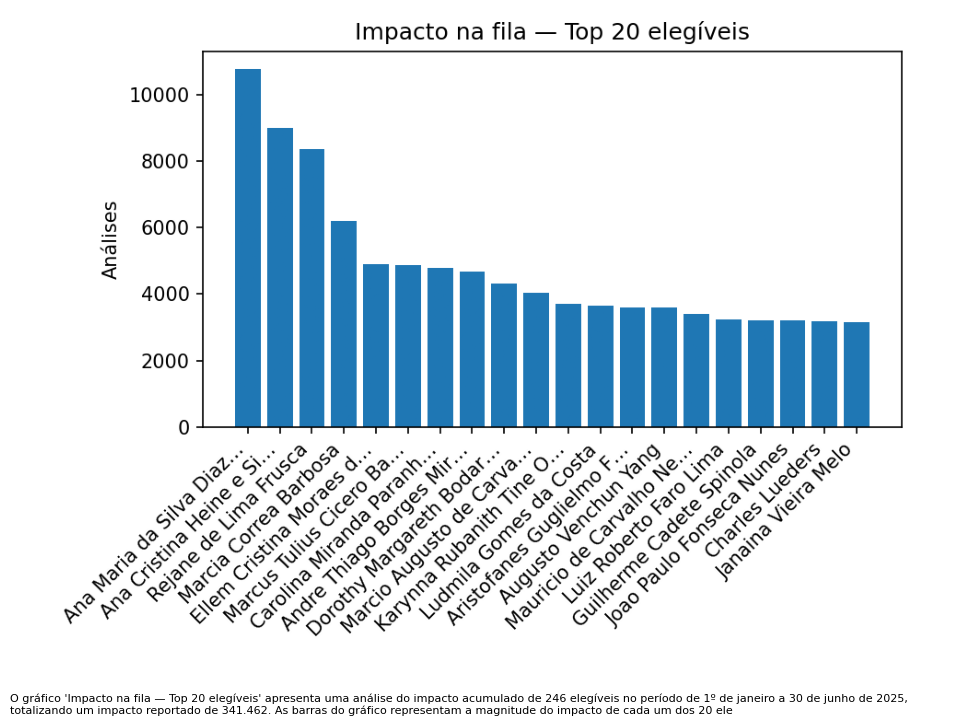
\includegraphics[width=.9\linewidth]{/home/gustavodetarso/Documentos/atestmed-defender/graphs_and_tables/exports/relatorio_fluxo_b_2025-01-01_a_2025-06-30_impacto_top20.png}
\end{center}
O gráfico 'Impacto na fila — Top 20 elegíveis' apresenta uma análise do impacto acumulado de 246 elegíveis no período de 1º de janeiro a 30 de junho de 2025, totalizando um impacto reportado de 341.462. As barras do gráfico representam a magnitude do impacto de cada um dos 20 elegíveis mais significativos, permitindo identificar quais têm maior contribuição para o total. A leitura das barras indica uma concentração de impacto, onde os primeiros colocados no ranking apresentam valores significativamente superiores aos demais, sugerindo que uma parte considerável do impacto total é gerada por um número reduzido de elegíveis. Essa característica pode ser interpretada como uma cauda longa, onde a maioria dos elegíveis tem um impacto menor, mas ainda assim relevante. Para a gestão, essa informação é crucial para priorizar ações e alocação de recursos, focando nos elegíveis que demonstram maior potencial de impacto, ao mesmo tempo em que se considera estratégias para aumentar a eficiência dos demais, garantindo uma abordagem equilibrada e eficaz na gestão do impacto.
\begin{center}
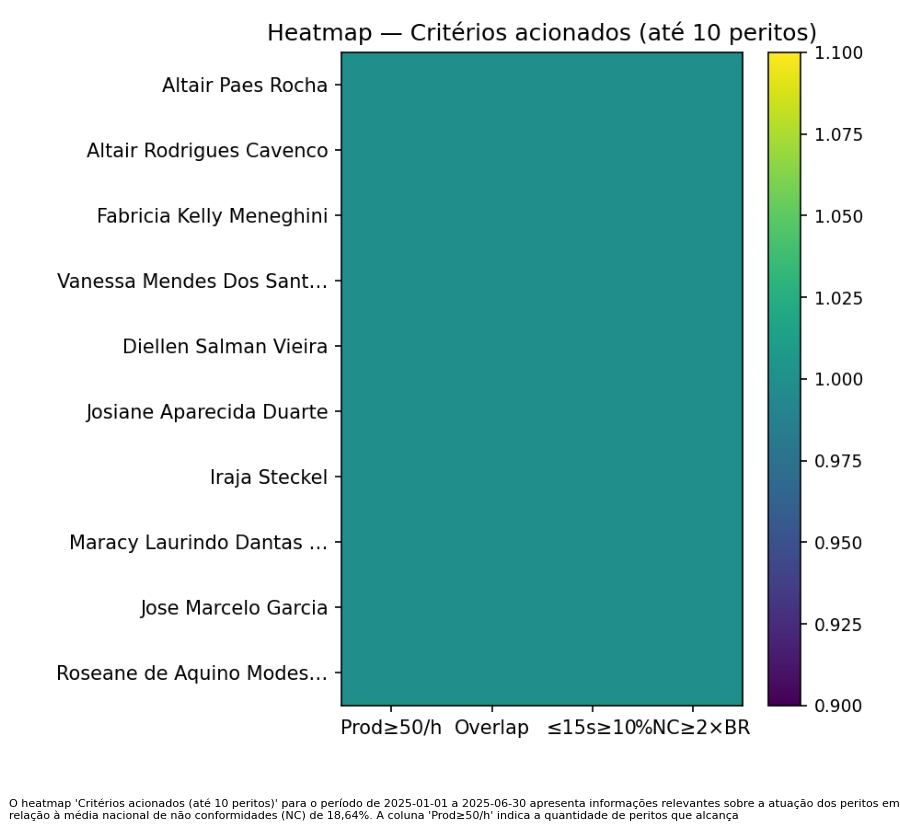
\includegraphics[width=.9\linewidth]{/home/gustavodetarso/Documentos/atestmed-defender/graphs_and_tables/exports/relatorio_fluxo_b_2025-01-01_a_2025-06-30_heatmap_score_flags.png}
\end{center}
O heatmap 'Critérios acionados (até 10 peritos)' para o período de 2025-01-01 a 2025-06-30 apresenta informações relevantes sobre a atuação dos peritos em relação à média nacional de não conformidades (NC) de 18,64\%. A coluna 'Prod≥50/h' indica a quantidade de peritos que alcançaram uma produtividade mínima de 50 horas, sugerindo eficiência no trabalho. A coluna 'Overlap' refere-se à sobreposição de casos analisados por diferentes peritos, o que pode indicar redundância ou colaboração. A coluna '≤15s≥10' mostra a quantidade de laudos que foram emitidos em menos de 15 segundos, sinalizando possíveis preocupações com a qualidade da análise. Por fim, a coluna '\%NC≥2×BR' indica a porcentagem de laudos com não conformidades que são pelo menos duas vezes superiores à média do Brasil, o que pode ser um indicativo de problemas mais graves. Na prática, é importante priorizar a análise de peritos com alta taxa de NC e baixa produtividade, além de investigar casos com alta sobreposição e laudos emitidos rapidamente, a fim de garantir a qualidade e a eficácia dos processos.
\begin{center}
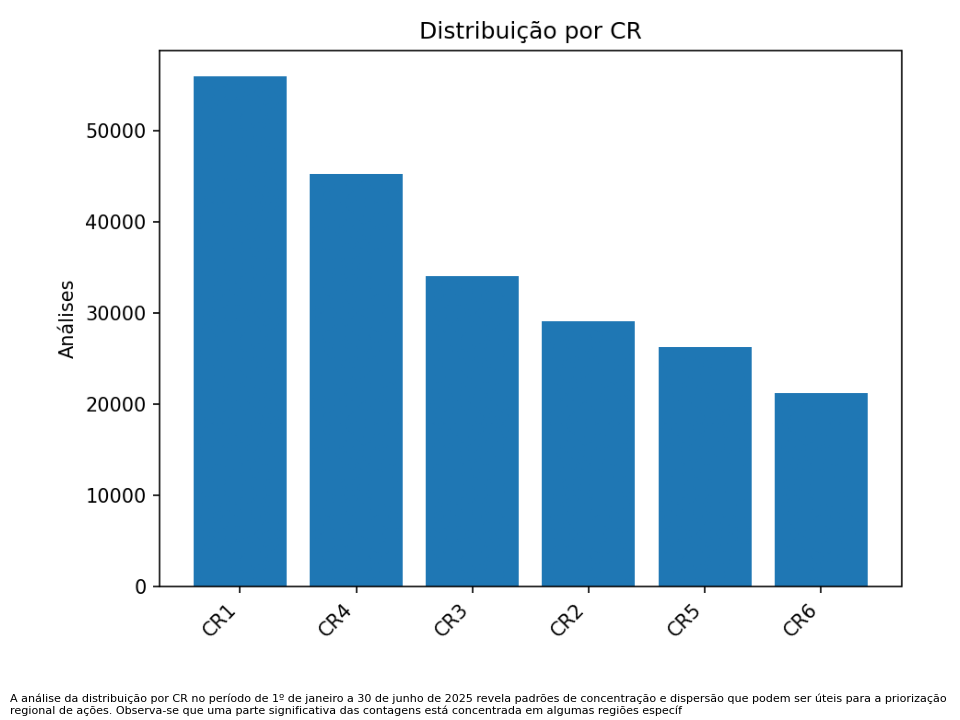
\includegraphics[width=.9\linewidth]{/home/gustavodetarso/Documentos/atestmed-defender/graphs_and_tables/exports/relatorio_fluxo_b_2025-01-01_a_2025-06-30_dist_por_CR.png}
\end{center}
A análise da distribuição por CR no período de 1º de janeiro a 30 de junho de 2025 revela padrões de concentração e dispersão que podem ser úteis para a priorização regional de ações. Observa-se que uma parte significativa das contagens está concentrada em algumas regiões específicas, indicando que essas áreas podem demandar atenção diferenciada em termos de recursos e políticas públicas. Por outro lado, a dispersão em outras regiões sugere que há uma necessidade de monitoramento contínuo, pois pode haver subnotificações ou falta de acesso a serviços. A visualização dessa distribuição permite identificar não apenas onde estão as maiores demandas, mas também onde as intervenções podem ser mais eficazes. Assim, gestores podem utilizar essas informações para direcionar esforços e recursos de forma mais estratégica, priorizando regiões com maior concentração de casos e, ao mesmo tempo, não negligenciando áreas com menor incidência, mas que podem apresentar riscos ocultos. Essa abordagem pode contribuir para uma gestão mais equilibrada e eficiente, alinhando ações às realidades locais.
\begin{center}
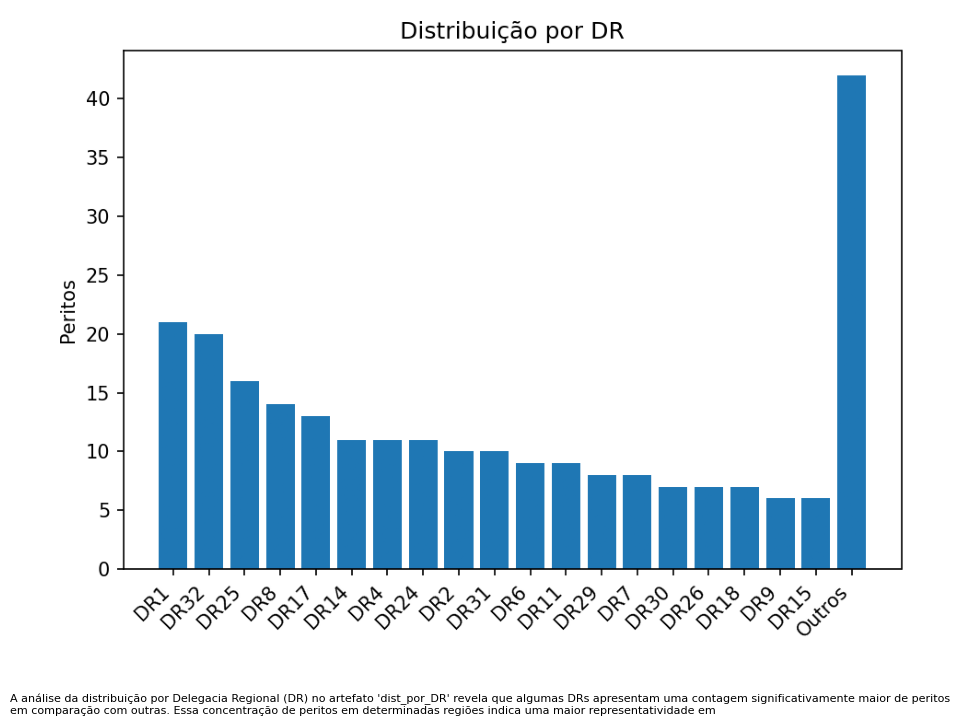
\includegraphics[width=.9\linewidth]{/home/gustavodetarso/Documentos/atestmed-defender/graphs_and_tables/exports/relatorio_fluxo_b_2025-01-01_a_2025-06-30_dist_por_DR.png}
\end{center}
A análise da distribuição por Delegacia Regional (DR) no artefato 'dist\textsubscript{por}\textsubscript{DR}' revela que algumas DRs apresentam uma contagem significativamente maior de peritos em comparação com outras. Essa concentração de peritos em determinadas regiões indica uma maior representatividade em áreas específicas, o que pode estar relacionado a fatores como a demanda por serviços periciais, a complexidade dos casos ou a infraestrutura disponível. As DRs com maior número de peritos podem ser consideradas prioritárias para a alocação de recursos e para o desenvolvimento de estratégias operacionais, uma vez que a eficiência no atendimento e a qualidade dos serviços prestados podem ser otimizadas nessas localidades. Por outro lado, as DRs com menor contagem de peritos podem necessitar de atenção especial para garantir que a cobertura pericial seja adequada e que a demanda da população seja atendida de forma eficaz. Assim, essa distribuição orienta a definição de focos operacionais e a necessidade de ajustes na gestão de recursos humanos nas diferentes DRs.
\begin{center}
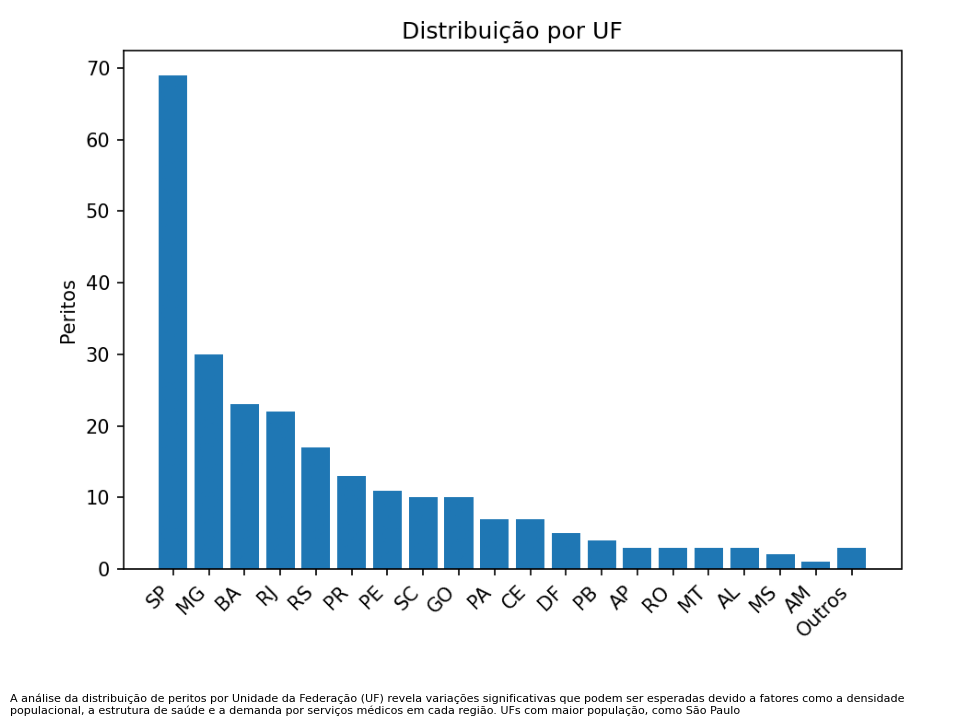
\includegraphics[width=.9\linewidth]{/home/gustavodetarso/Documentos/atestmed-defender/graphs_and_tables/exports/relatorio_fluxo_b_2025-01-01_a_2025-06-30_dist_por_UF.png}
\end{center}
A análise da distribuição de peritos por Unidade da Federação (UF) revela variações significativas que podem ser esperadas devido a fatores como a densidade populacional, a estrutura de saúde e a demanda por serviços médicos em cada região. UFs com maior população, como São Paulo e Minas Gerais, tendem a apresentar um número elevado de peritos, refletindo a necessidade de atendimento a uma demanda maior. Por outro lado, estados menos populosos, como Roraima ou Acre, podem ter uma contagem inferior, o que pode indicar uma cobertura insuficiente ou a necessidade de estratégias de mobilidade para garantir o acesso à perícia médica. Essas diferenças, tanto esperadas quanto inesperadas, são cruciais para a governança local, pois permitem que gestores identifiquem áreas que necessitam de mais recursos ou de uma melhor distribuição de profissionais, contribuindo para a equidade no acesso aos serviços de saúde e para a eficiência na gestão pública. A análise contínua desses dados pode informar políticas que visem a otimização da alocação de peritos, melhorando a resposta às necessidades da população.
\begin{center}
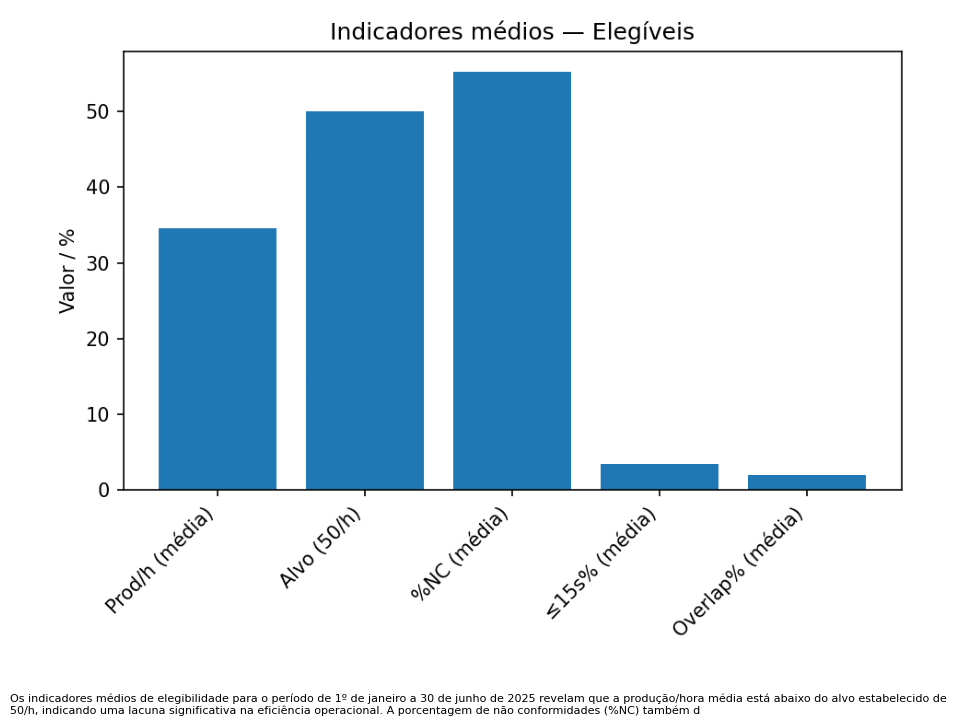
\includegraphics[width=.9\linewidth]{/home/gustavodetarso/Documentos/atestmed-defender/graphs_and_tables/exports/relatorio_fluxo_b_2025-01-01_a_2025-06-30_indicadores_medios.png}
\end{center}
Os indicadores médios de elegibilidade para o período de 1º de janeiro a 30 de junho de 2025 revelam que a produção/hora média está abaixo do alvo estabelecido de 50/h, indicando uma lacuna significativa na eficiência operacional. A porcentagem de não conformidades (\%NC) também deve ser monitorada, pois um aumento nesse indicador pode sinalizar problemas na qualidade dos processos. O tempo de resposta (≤15s\%) é um aspecto crítico, e se os dados mostrarem que a maioria das respostas excede esse limite, isso pode impactar negativamente a satisfação do usuário e a eficácia do serviço. Além disso, o Overlap\% deve ser avaliado, pois um alto percentual pode indicar redundâncias ou ineficiências nos processos, aumentando o risco de erros e retrabalho. Essas lacunas em relação ao alvo e os riscos operacionais associados exigem uma análise mais aprofundada e a implementação de medidas corretivas para garantir que os objetivos de desempenho sejam alcançados e a qualidade dos serviços prestados seja mantida.
\begin{center}
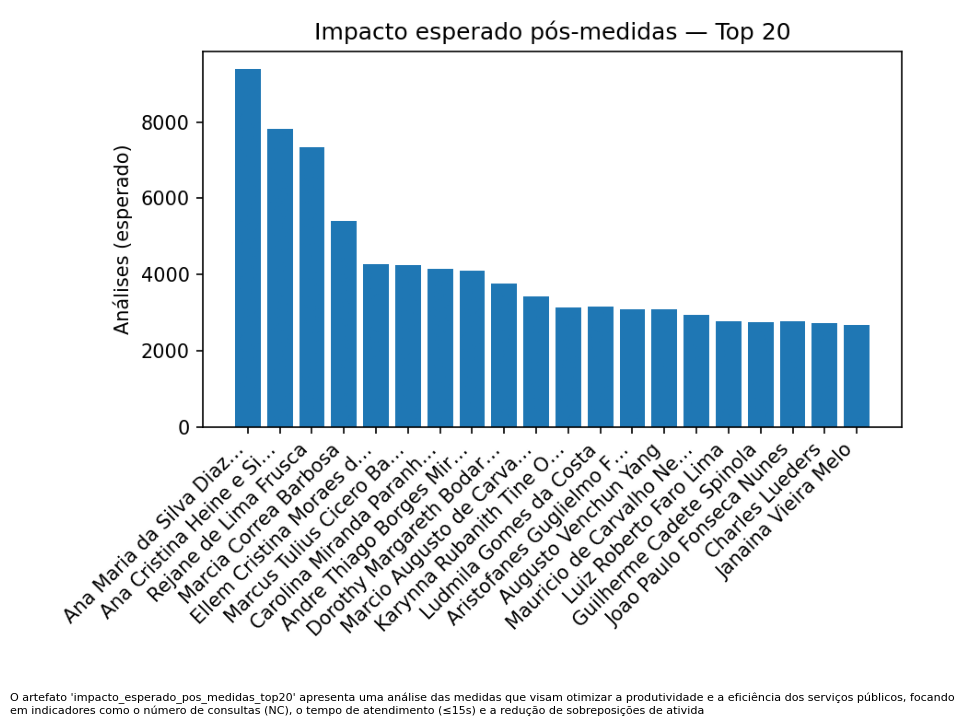
\includegraphics[width=.9\linewidth]{/home/gustavodetarso/Documentos/atestmed-defender/graphs_and_tables/exports/relatorio_fluxo_b_2025-01-01_a_2025-06-30_impacto_esperado_pos_medidas_top20.png}
\end{center}
O artefato 'impacto\textsubscript{esperado}\textsubscript{pos}\textsubscript{medidas}\textsubscript{top20}' apresenta uma análise das medidas que visam otimizar a produtividade e a eficiência dos serviços públicos, focando em indicadores como o número de consultas (NC), o tempo de atendimento (≤15s) e a redução de sobreposições de atividades. A lógica por trás dessas medidas é que a melhoria na produtividade e na redução do tempo de espera pode resultar em um atendimento mais ágil e eficaz, beneficiando a população. As hipóteses subjacentes incluem a premissa de que a implementação dessas ações levará a um aumento na satisfação do usuário e na eficiência operacional. No entanto, é importante reconhecer as limitações dessa análise, como a variabilidade nos contextos locais e a dificuldade em mensurar impactos diretos. Para priorizar ações de curto prazo, recomenda-se focar nas medidas que apresentam maior potencial de impacto imediato, considerando a viabilidade de implementação e a capacidade de monitoramento dos resultados, garantindo assim uma gestão mais eficiente e responsiva às necessidades da população.
\begin{center}
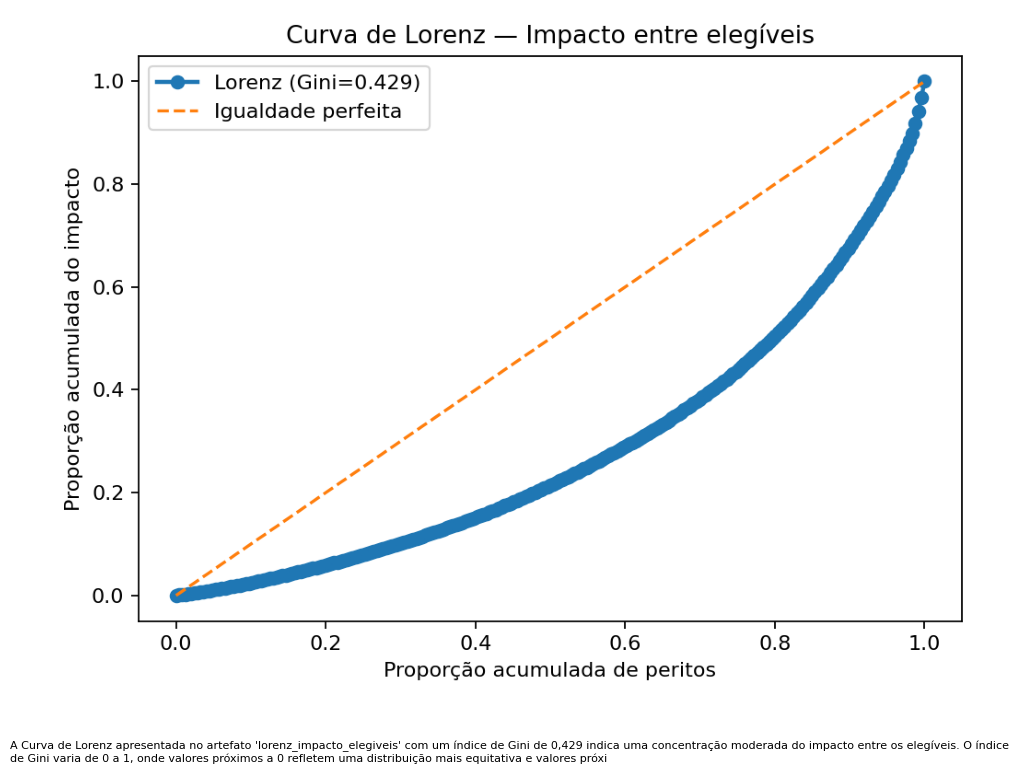
\includegraphics[width=.9\linewidth]{/home/gustavodetarso/Documentos/atestmed-defender/graphs_and_tables/exports/relatorio_fluxo_b_2025-01-01_a_2025-06-30_lorenz_impacto_elegiveis.png}
\end{center}
A Curva de Lorenz apresentada no artefato 'lorenz\textsubscript{impacto}\textsubscript{elegiveis}' com um índice de Gini de 0,429 indica uma concentração moderada do impacto entre os elegíveis. O índice de Gini varia de 0 a 1, onde valores próximos a 0 refletem uma distribuição mais equitativa e valores próximos a 1 indicam maior concentração. Neste caso, o valor de 0,429 sugere que há uma desigualdade considerável na distribuição do impacto, o que implica que uma parte dos elegíveis está recebendo uma proporção significativa dos benefícios ou recursos disponíveis. Essa curvatura da curva de Lorenz demonstra que as prioridades na alocação de recursos podem estar favorecendo determinados grupos ou indivíduos, o que pode ser um indicativo para a gestão pública revisar suas estratégias de intervenção. A análise sugere a necessidade de um olhar mais atento para garantir que o impacto seja distribuído de maneira mais equitativa, promovendo uma maior inclusão e eficácia nas políticas públicas direcionadas aos elegíveis.
\begin{center}
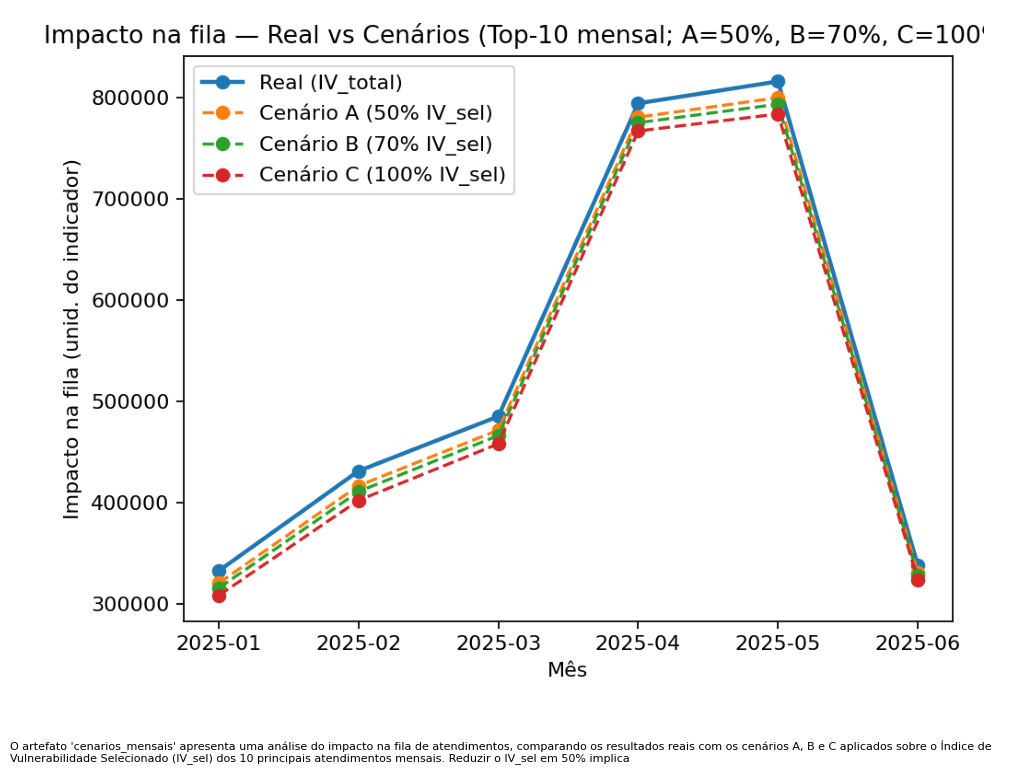
\includegraphics[width=.9\linewidth]{/home/gustavodetarso/Documentos/atestmed-defender/graphs_and_tables/exports/relatorio_fluxo_b_2025-01-01_a_2025-06-30_cenarios_mensais.png}
\end{center}
O artefato 'cenarios\textsubscript{mensais}' apresenta uma análise do impacto na fila de atendimentos, comparando os resultados reais com os cenários A, B e C aplicados sobre o Índice de Vulnerabilidade Selecionado (IV\textsubscript{sel}) dos 10 principais atendimentos mensais. Reduzir o IV\textsubscript{sel} em 50\% implica que a fila de atendimentos seria significativamente diminuída, resultando em um tempo de espera menor e potencialmente melhorando a eficiência do serviço. Uma redução de 70\% sugere um impacto ainda mais expressivo, podendo levar a uma fila quase inexistente, o que favorece a agilidade no atendimento. Por fim, uma redução de 100\% indica a eliminação total da fila, o que é um cenário ideal, mas pode não ser viável na prática. As simulações desses cenários orientam a definição de metas realistas e alcançáveis, permitindo que gestores avaliem diferentes estratégias de intervenção e alocação de recursos para melhorar o atendimento e reduzir a demanda reprimida. Assim, essas análises são fundamentais para a tomada de decisões informadas na gestão pública.
\begin{center}
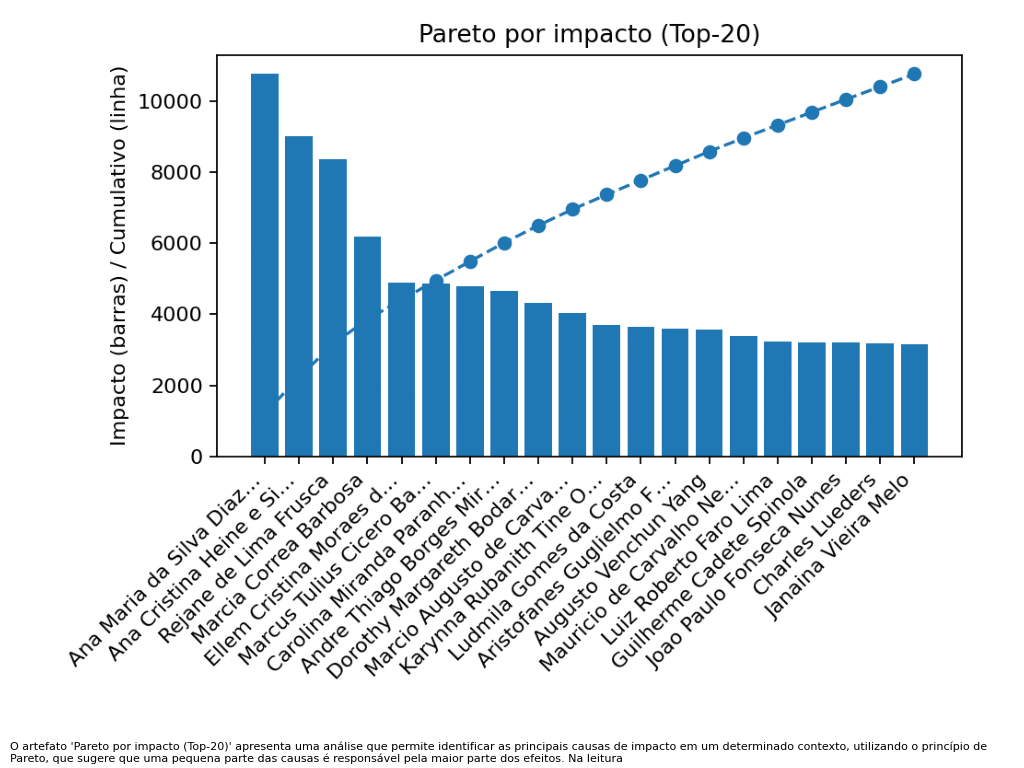
\includegraphics[width=.9\linewidth]{/home/gustavodetarso/Documentos/atestmed-defender/graphs_and_tables/exports/relatorio_fluxo_b_2025-01-01_a_2025-06-30_pareto_impacto.png}
\end{center}
O artefato 'Pareto por impacto (Top-20)' apresenta uma análise que permite identificar as principais causas de impacto em um determinado contexto, utilizando o princípio de Pareto, que sugere que uma pequena parte das causas é responsável pela maior parte dos efeitos. Na leitura do gráfico, as barras representam a magnitude de cada causa, enquanto a linha cumulativa indica a porcentagem acumulada do impacto total. Essa visualização facilita a identificação das causas mais relevantes, permitindo que gestores direcionem esforços para as questões que realmente influenciam os resultados. O ponto de corte, geralmente estabelecido em 80\% do impacto acumulado, serve como um guia para priorizar ações, focando nas causas que estão entre as mais significativas. Ao concentrar recursos e estratégias nas principais causas identificadas, é possível otimizar a gestão e potencializar os resultados, garantindo uma abordagem mais eficaz na resolução de problemas. Essa análise é fundamental para a tomada de decisões informadas e para a melhoria contínua dos processos.
\begin{center}
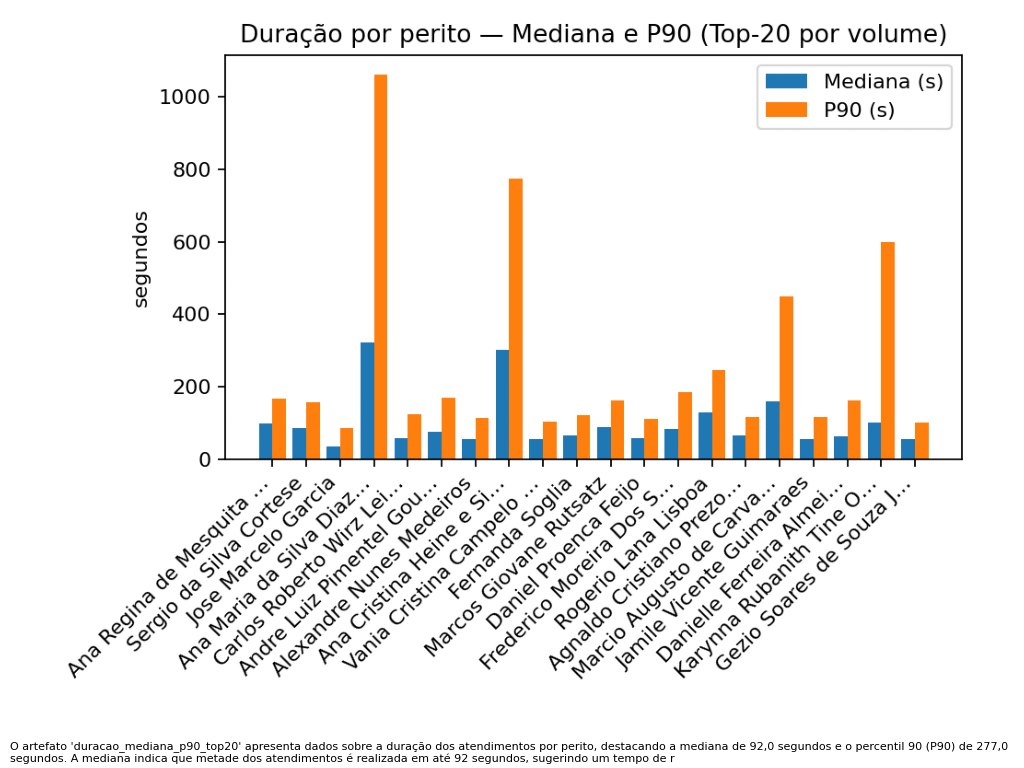
\includegraphics[width=.9\linewidth]{/home/gustavodetarso/Documentos/atestmed-defender/graphs_and_tables/exports/relatorio_fluxo_b_2025-01-01_a_2025-06-30_duracao_mediana_p90_top20.png}
\end{center}
O artefato 'duracao\textsubscript{mediana}\textsubscript{p90}\textsubscript{top20}' apresenta dados sobre a duração dos atendimentos por perito, destacando a mediana de 92,0 segundos e o percentil 90 (P90) de 277,0 segundos. A mediana indica que metade dos atendimentos é realizada em até 92 segundos, sugerindo um tempo de resposta relativamente eficiente para a maioria dos casos. No entanto, o P90, que representa o tempo que 90\% dos atendimentos não ultrapassam, revela uma variabilidade significativa, com alguns atendimentos levando até 277 segundos. Essa discrepância entre a mediana e o P90 sugere a presença de casos mais complexos ou situações que demandam mais tempo, o que pode impactar a fila de atendimentos e a capacidade operacional. A gestão dessa variabilidade é crucial, pois pode indicar a necessidade de revisão de processos ou capacitação adicional para os peritos, visando otimizar o fluxo de atendimento e reduzir o tempo de espera para os usuários. Portanto, a análise desses dados é fundamental para identificar oportunidades de melhoria na eficiência do serviço prestado.

\section{Pareto por impacto}
\label{sec:org66066af}
\begin{center}
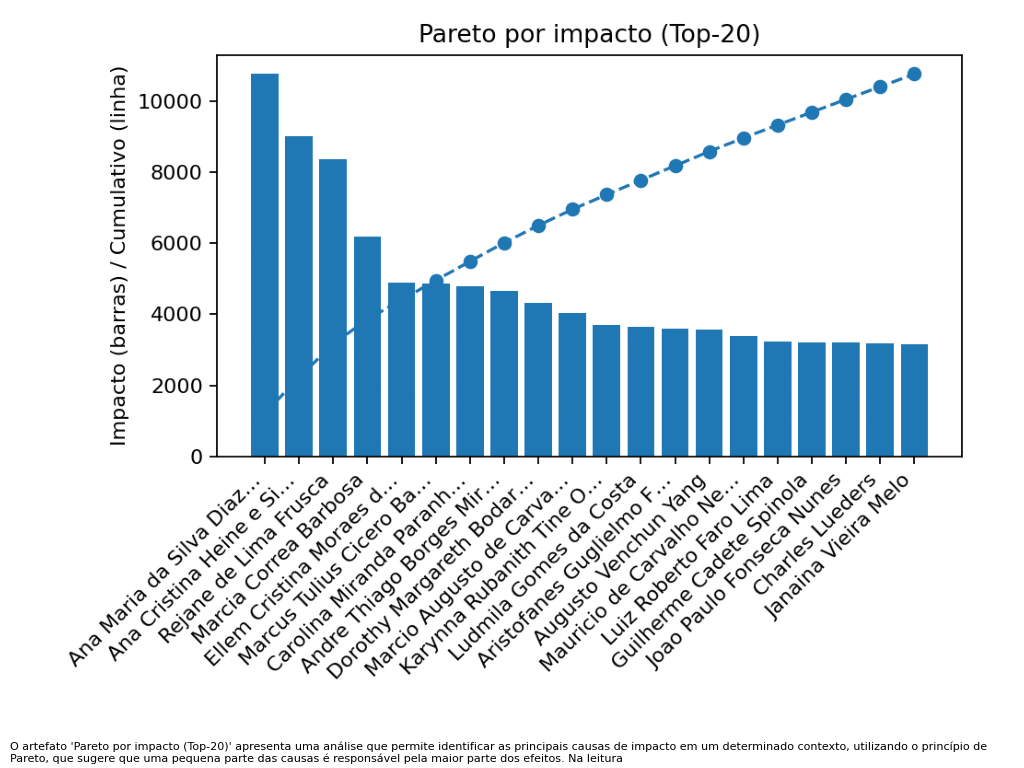
\includegraphics[width=.9\linewidth]{/home/gustavodetarso/Documentos/atestmed-defender/graphs_and_tables/exports/relatorio_fluxo_b_2025-01-01_a_2025-06-30_pareto_impacto.png}
\end{center}

\begingroup\scriptsize
\begin{center}
\begin{tabular}{rlrrr}
Rank & Perito & Impacto & \% & Cumul\%\\
\hline
1 & Ana Maria da Silva Diaz… & 10769 & 3.15 & 3.15\\
2 & Ana Cristina Heine e Si… & 9008 & 2.64 & 5.79\\
3 & Rejane de Lima Frusca & 8367 & 2.45 & 8.24\\
4 & Marcia Correa Barbosa & 6200 & 1.82 & 10.06\\
5 & Ellem Cristina Moraes d… & 4886 & 1.43 & 11.49\\
6 & Marcus Tulius Cicero Ba… & 4858 & 1.42 & 12.91\\
7 & Carolina Miranda Paranh… & 4784 & 1.4 & 14.31\\
8 & Andre Thiago Borges Mir… & 4672 & 1.37 & 15.68\\
9 & Dorothy Margareth Bodar… & 4329 & 1.27 & 16.95\\
10 & Marcio Augusto de Carva… & 4041 & 1.18 & 18.13\\
\end{tabular}
\end{center}
\endgroup
O artefato 'Pareto por impacto (Top-20)' apresenta uma análise que permite identificar as principais causas de impacto em um determinado contexto, organizando-as em ordem decrescente. As barras representam a magnitude de cada causa, enquanto a linha cumulativa indica a porcentagem acumulada do impacto total. Essa visualização facilita a identificação das causas mais significativas, permitindo que gestores priorizem ações corretivas. O ponto de corte, geralmente estabelecido em 80\% do impacto acumulado, serve como um guia para focar nas causas que, se abordadas, podem resultar em melhorias substanciais. Ao concentrar esforços nas principais causas identificadas, é possível otimizar recursos e aumentar a eficácia das intervenções. A leitura conjunta das barras e da linha cumulativa é essencial para uma compreensão completa do cenário, pois revela não apenas quais são os problemas mais críticos, mas também a proporção do impacto que cada um representa em relação ao total. Essa abordagem orientada por dados é fundamental para a tomada de decisões informadas na gestão pública.

\section{Cenários (conforme melhorias.org)}
\label{sec:orgb360339}
Aplicação das reduções A/B/C sobre IV\textsubscript{sel} (Top-10 mensal).
\begingroup\scriptsize
\begin{center}
\begin{tabular}{rrrrrrrrrrrr}
Mes & IV\textsubscript{total} & IV\textsubscript{sel} & Cen\textsubscript{A} & Red\textsubscript{A} & Red\textsubscript{A}\_\% & Cen\textsubscript{B} & Red\textsubscript{B} & Red\textsubscript{B}\_\% & Cen\textsubscript{C} & Red\textsubscript{C} & Red\textsubscript{C}\_\%\\
\hline
2025-01 & 332611 & 24255 & 320484 & 12128 & 3.65 & 315632 & 16979 & 5.1 & 308356 & 24255 & 7.29\\
2025-02 & 431248 & 29008 & 416744 & 14504 & 3.36 & 410943 & 20306 & 4.71 & 402240 & 29008 & 6.73\\
2025-03 & 485152 & 27065 & 471620 & 13533 & 2.79 & 466207 & 18946 & 3.91 & 458087 & 27065 & 5.58\\
2025-04 & 794251 & 27295 & 780604 & 13647 & 1.72 & 775145 & 19106 & 2.41 & 766956 & 27295 & 3.44\\
2025-05 & 815889 & 32130 & 799824 & 16065 & 1.97 & 793398 & 22491 & 2.76 & 783759 & 32130 & 3.94\\
2025-06 & 338029 & 14091 & 330983 & 7046 & 2.08 & 328165 & 9864 & 2.92 & 323938 & 14091 & 4.17\\
\textbf{Total} & 3197181 & 153845 & — & 76923 & 2.41 & — & 107692 & 3.37 & — & 153845 & 4.81\\
\end{tabular}
\end{center}
\endgroup
A tabela 'Cenários mensais (CSV)' apresenta informações sobre os índices de variação (IV\textsubscript{total} e IV\textsubscript{sel}) e as reduções por rótulo ao longo dos meses. O IV\textsubscript{total} representa a variação acumulada ao longo do período analisado, enquanto o IV\textsubscript{sel} reflete a variação específica de um subconjunto de dados, permitindo uma comparação mais focada. Os deltas mensais indicam a diferença entre os valores de um mês e o mês anterior, possibilitando a identificação de tendências e flutuações no desempenho. Para interpretar esses deltas, é importante observar se os valores são positivos ou negativos, o que indica aumento ou diminuição, respectivamente. Além disso, a análise das reduções por rótulo fornece insights sobre quais categorias estão apresentando maior ou menor desempenho, contribuindo para uma avaliação mais detalhada das áreas que podem necessitar de atenção ou intervenção. Assim, a combinação dessas métricas permite uma compreensão mais abrangente do cenário em questão, facilitando a tomada de decisões informadas.

\section{Propostas}
\label{sec:orgc2a2c1e}
\section{Medidas propostas (foco nos 10 piores por mês)}
\label{sec:orgd284879}
As medidas abaixo visam reduzir a captura maliciosa do fluxo por parte do \textbf{grupo focal} (top-10 piores/mês), preservando a boa atuação da maioria:

\begin{enumerate}
\item \textbf{Throttle adaptativo de fila}: diminui o \emph{throughput} do perito quando disparar \textbf{qualquer} gatilho de risco (janelas móveis de 5, 15, 60 min).
\item \textbf{Cool-down obrigatório} pós-gatilho: pausas mínimas progressivas (p.ex., 2, 5, 10 min) após eventos de sobreposição ou explosões de produtividade.
\item \textbf{Hard-cap de paralelismo}: impedir submissões concorrentes do mesmo perito em janelas curtas.
\item \textbf{Revalidação obrigatória} para laudos fora do padrão (≤15s; >50/h; não-conformidade anômala): formulário de double-check e anexos.
\item \textbf{Escalonamento automát.} para auditoria: envio de amostra estratificada dos laudos do grupo focal para parecer técnico independente.
\item \textbf{Score v2 embutido na UI}: transparência do risco (perito vê o próprio score; gestores veem heatmap de gatilhos).
\item \textbf{Penalidade de roteamento}: reduzir a alocação de novos casos ao perito enquanto perdurar estado de risco.
\item \textbf{Alertas e trilhas}: notificações em tempo real para coordenação; trilhas de auditoria replicáveis.
\item \textbf{Educação + Termo de Compromisso}: para reincidências, treino dirigido e aceite formal de boas práticas.
\item \textbf{Corte administrativo escalonado}: suspensão temporária se KPIs não retornarem ao \emph{baseline}.
\end{enumerate}

Arquivo (plano de ação): \href{file:///home/gustavodetarso/Documentos/atestmed-defender/graphs\_and\_tables/exports/relatorio\_fluxo\_b\_2025-01-01\_a\_2025-06-30\_plano\_acao.csv}{plano\textsubscript{acao.csv}}
O artefato 'plano\textsubscript{acao}\textsubscript{csv}' apresenta um plano de ação estruturado que visa otimizar processos e resultados em gestão pública. As colunas de "ganho esperado" e "gargalos" são fundamentais para a análise e acompanhamento das ações propostas. A coluna de "ganho esperado" indica os resultados positivos que se espera alcançar com a implementação de cada ação, permitindo priorizar iniciativas com maior impacto. Já a coluna de "gargalos" identifica os obstáculos que podem dificultar a execução das ações, possibilitando um planejamento mais realista e a adoção de medidas mitigadoras. Para utilizar esse plano na rotina de acompanhamento, é essencial monitorar periodicamente o progresso das ações, avaliando se os ganhos esperados estão sendo alcançados e se os gargalos identificados estão sendo efetivamente tratados. Essa prática permite ajustes nas estratégias e garante que os objetivos do plano sejam cumpridos de forma eficiente, contribuindo para a melhoria contínua dos serviços públicos.

\section{Explicações e Metodologia}
\label{sec:orgf9ac965}
\#\#\# Métricas do Projeto ATESTMED

\begin{enumerate}
\item \textbf{\textbf{\%NC (Percentual de Não Conformidades)}}: Esta métrica representa a porcentagem de casos que não atendem aos critérios estabelecidos. No período analisado, o percentual de não conformidades foi de aproximadamente \textbf{\textbf{55.18\%}}. Isso indica que mais da metade dos casos analisados apresentaram algum tipo de não conformidade.

\item \textbf{\textbf{Prod/h (Produção por Hora)}}: Refere-se à quantidade média de casos processados por hora. A média de produção foi de \textbf{\textbf{34.62 casos/hora}}, o que fornece uma visão sobre a eficiência do fluxo de trabalho.

\item \textbf{\textbf{≤15s (Percentual de Casos Processados em até 15 segundos)}}: Esta métrica indica a porcentagem de casos que foram processados em um tempo igual ou inferior a 15 segundos. O percentual registrado foi de \textbf{\textbf{3.43\%}}, sugerindo que a maioria dos casos leva mais tempo para ser processada.

\item \textbf{\textbf{Overlap (Sobreposição)}}: Refere-se à porcentagem de casos que se sobrepõem em diferentes categorias ou critérios. O percentual de sobreposição foi de \textbf{\textbf{2.01\%}}, indicando que há uma pequena quantidade de casos que se encaixam em múltiplas categorias.

\item \textbf{\textbf{Score v2}}: Embora não haja um valor específico fornecido para o Score v2, ele é uma métrica que pode ser utilizada para avaliar a qualidade ou a relevância dos casos analisados, possivelmente levando em consideração múltiplos fatores.
\end{enumerate}

\#\#\# Regras do Fluxo B

O Fluxo B é um processo que envolve a análise de casos elegíveis, onde são aplicadas regras específicas para determinar a conformidade e a eficiência do fluxo de trabalho. As regras podem incluir critérios de elegibilidade, prazos de processamento e a necessidade de revisões adicionais para casos que não atendem aos padrões estabelecidos.

\#\#\# Cálculo do 'Impacto na Fila'

O impacto na fila é calculado com base na soma dos impactos dos casos elegíveis. No período analisado, a soma do impacto foi de \textbf{\textbf{341,461.78}}. Este valor pode ser utilizado para priorizar casos que têm um impacto maior na operação e na eficiência do fluxo de trabalho.

\#\#\# Comentários sobre Gráficos e Cenários Probabilísticos

Os gráficos gerados para o período analisado fornecem uma visão abrangente sobre o desempenho do Fluxo B. Eles incluem:

\begin{itemize}
\item \textbf{\textbf{Impacto Top 20}}: Identifica os casos com maior impacto, permitindo focar em melhorias onde são mais necessárias.
\item \textbf{\textbf{Heatmap de Score e Flags}}: Ajuda a visualizar a distribuição de scores e a identificação de padrões de não conformidade.
\item \textbf{\textbf{Distribuições por CR, DR e UF}}: Permitem entender como as variáveis demográficas e regionais afetam o desempenho.
\item \textbf{\textbf{Cenários Mensais}}: Avaliam diferentes hipóteses de redução de não conformidades, com reduções propostas de 0.5, 0.7 e 1.0, permitindo simulações de impacto.
\end{itemize}

\#\#\#\# Cenários e Hipóteses

Os cenários A, B e C representam diferentes estratégias de redução de não conformidades. A hipótese é que a implementação de medidas corretivas pode reduzir significativamente o percentual de não conformidades e melhorar a eficiência do fluxo de trabalho.

\#\#\#\# Limitações

As limitações incluem a dependência de dados históricos, que podem não refletir mudanças futuras nas operações ou na legislação. Além disso, a análise pode ser afetada por variáveis externas não consideradas nos dados.

\#\#\#\# Recomendações

\begin{enumerate}
\item \textbf{\textbf{Foco nas Não Conformidades}}: Implementar medidas corretivas para os casos que mais contribuem para o percentual de não conformidades.
\item \textbf{\textbf{Aumentar a Eficiência}}: Buscar formas de aumentar a produção por hora, possivelmente através de treinamentos ou melhorias nos processos.
\item \textbf{\textbf{Monitoramento Contínuo}}: Continuar a monitorar as métricas e ajustar as estratégias conforme necessário, utilizando os dados dos gráficos e cenários para informar decisões.
\end{enumerate}

Essas análises e recomendações podem ajudar a otimizar o Fluxo B e melhorar a eficiência geral do projeto ATESTMED.

\section{Apêndice — Tabela completa de peritos (arquivo)}
\label{sec:org078f271}
\href{file:///home/gustavodetarso/Documentos/atestmed-defender/graphs\_and\_tables/exports/relatorio\_fluxo\_b\_2025-01-01\_a\_2025-06-30\_FULL.csv}{relatorio\textsubscript{fluxo}\textsubscript{b}\textsubscript{2025}-01-01\textsubscript{a}\textsubscript{2025}-06-30\textsubscript{FULL.csv}}
A 'Tabela completa de peritos' presente no artefato 'tabela\textsubscript{full}\textsubscript{csv}' é uma ferramenta essencial para a auditoria e análise de dados no contexto do ATESTMED. Essa tabela reúne informações detalhadas sobre os peritos, incluindo suas especializações, registros e histórico de atuação, o que permite uma verificação minuciosa da conformidade e da qualificação dos profissionais envolvidos. A auditoria pode se beneficiar dessa tabela ao realizar um drill-down, possibilitando a investigação de casos específicos, identificação de padrões de atuação e análise de eventuais inconsistências nos dados. Além disso, a tabela facilita checagens de consistência, permitindo cruzar informações com outras bases de dados e verificar a veracidade das informações apresentadas. Dessa forma, a 'Tabela completa de peritos' não apenas apoia a transparência e a responsabilidade na gestão pública, mas também contribui para a melhoria contínua dos processos de avaliação e supervisão dos serviços prestados.

\section{Arquivos gerados}
\label{sec:org668ffcd}
\begin{itemize}
\item \href{file:///home/gustavodetarso/Documentos/atestmed-defender/graphs\_and\_tables/exports/relatorio\_fluxo\_b\_2025-01-01\_a\_2025-06-30.org}{Relatório ORG}
\item \href{file:///home/gustavodetarso/Documentos/atestmed-defender/graphs\_and\_tables/exports/pdf/relatorio\_fluxo\_b\_2025-01-01\_a\_2025-06-30.pdf}{Relatório PDF}
\item \href{file:///home/gustavodetarso/Documentos/atestmed-defender/graphs\_and\_tables/exports/relatorio\_fluxo\_b\_2025-01-01\_a\_2025-06-30.csv}{CSV principal (ranking)}
\item \href{file:///home/gustavodetarso/Documentos/atestmed-defender/graphs\_and\_tables/exports/relatorio\_fluxo\_b\_2025-01-01\_a\_2025-06-30\_FULL.csv}{CSV completo}
\item \href{file:///home/gustavodetarso/Documentos/atestmed-defender/graphs\_and\_tables/exports/relatorio\_fluxo\_b\_2025-01-01\_a\_2025-06-30\_plano\_acao.csv}{Plano de ação}
\item \href{file:///home/gustavodetarso/Documentos/atestmed-defender/graphs\_and\_tables/exports/relatorio\_fluxo\_b\_2025-01-01\_a\_2025-06-30\_cenarios\_mensais.csv}{Cenários (CSV)}
\item \href{file:///home/gustavodetarso/Documentos/atestmed-defender/graphs\_and\_tables/exports/relatorio\_fluxo\_b\_2025-01-01\_a\_2025-06-30\_cenarios\_mensais.png}{Cenários (PNG)}
\item \href{file:///home/gustavodetarso/Documentos/atestmed-defender/graphs\_and\_tables/exports/relatorio\_fluxo\_b\_2025-01-01\_a\_2025-06-30\_impacto\_top20.png}{relatorio\textsubscript{fluxo}\textsubscript{b}\textsubscript{2025}-01-01\textsubscript{a}\textsubscript{2025}-06-30\textsubscript{impacto}\textsubscript{top20.png}}
\item \href{file:///home/gustavodetarso/Documentos/atestmed-defender/graphs\_and\_tables/exports/relatorio\_fluxo\_b\_2025-01-01\_a\_2025-06-30\_heatmap\_score\_flags.png}{relatorio\textsubscript{fluxo}\textsubscript{b}\textsubscript{2025}-01-01\textsubscript{a}\textsubscript{2025}-06-30\textsubscript{heatmap}\textsubscript{score}\textsubscript{flags.png}}
\item \href{file:///home/gustavodetarso/Documentos/atestmed-defender/graphs\_and\_tables/exports/relatorio\_fluxo\_b\_2025-01-01\_a\_2025-06-30\_dist\_por\_CR.png}{relatorio\textsubscript{fluxo}\textsubscript{b}\textsubscript{2025}-01-01\textsubscript{a}\textsubscript{2025}-06-30\textsubscript{dist}\textsubscript{por}\textsubscript{CR.png}}
\item \href{file:///home/gustavodetarso/Documentos/atestmed-defender/graphs\_and\_tables/exports/relatorio\_fluxo\_b\_2025-01-01\_a\_2025-06-30\_dist\_por\_DR.png}{relatorio\textsubscript{fluxo}\textsubscript{b}\textsubscript{2025}-01-01\textsubscript{a}\textsubscript{2025}-06-30\textsubscript{dist}\textsubscript{por}\textsubscript{DR.png}}
\item \href{file:///home/gustavodetarso/Documentos/atestmed-defender/graphs\_and\_tables/exports/relatorio\_fluxo\_b\_2025-01-01\_a\_2025-06-30\_dist\_por\_UF.png}{relatorio\textsubscript{fluxo}\textsubscript{b}\textsubscript{2025}-01-01\textsubscript{a}\textsubscript{2025}-06-30\textsubscript{dist}\textsubscript{por}\textsubscript{UF.png}}
\item \href{file:///home/gustavodetarso/Documentos/atestmed-defender/graphs\_and\_tables/exports/relatorio\_fluxo\_b\_2025-01-01\_a\_2025-06-30\_indicadores\_medios.png}{relatorio\textsubscript{fluxo}\textsubscript{b}\textsubscript{2025}-01-01\textsubscript{a}\textsubscript{2025}-06-30\textsubscript{indicadores}\textsubscript{medios.png}}
\item \href{file:///home/gustavodetarso/Documentos/atestmed-defender/graphs\_and\_tables/exports/relatorio\_fluxo\_b\_2025-01-01\_a\_2025-06-30\_impacto\_esperado\_pos\_medidas\_top20.png}{relatorio\textsubscript{fluxo}\textsubscript{b}\textsubscript{2025}-01-01\textsubscript{a}\textsubscript{2025}-06-30\textsubscript{impacto}\textsubscript{esperado}\textsubscript{pos}\textsubscript{medidas}\textsubscript{top20.png}}
\item \href{file:///home/gustavodetarso/Documentos/atestmed-defender/graphs\_and\_tables/exports/relatorio\_fluxo\_b\_2025-01-01\_a\_2025-06-30\_lorenz\_impacto\_elegiveis.png}{relatorio\textsubscript{fluxo}\textsubscript{b}\textsubscript{2025}-01-01\textsubscript{a}\textsubscript{2025}-06-30\textsubscript{lorenz}\textsubscript{impacto}\textsubscript{elegiveis.png}}
\item \href{file:///home/gustavodetarso/Documentos/atestmed-defender/graphs\_and\_tables/exports/relatorio\_fluxo\_b\_2025-01-01\_a\_2025-06-30\_cenarios\_mensais.png}{relatorio\textsubscript{fluxo}\textsubscript{b}\textsubscript{2025}-01-01\textsubscript{a}\textsubscript{2025}-06-30\textsubscript{cenarios}\textsubscript{mensais.png}}
\item \href{file:///home/gustavodetarso/Documentos/atestmed-defender/graphs\_and\_tables/exports/relatorio\_fluxo\_b\_2025-01-01\_a\_2025-06-30\_pareto\_impacto.png}{relatorio\textsubscript{fluxo}\textsubscript{b}\textsubscript{2025}-01-01\textsubscript{a}\textsubscript{2025}-06-30\textsubscript{pareto}\textsubscript{impacto.png}}
\item \href{file:///home/gustavodetarso/Documentos/atestmed-defender/graphs\_and\_tables/exports/relatorio\_fluxo\_b\_2025-01-01\_a\_2025-06-30\_duracao\_mediana\_p90\_top20.png}{relatorio\textsubscript{fluxo}\textsubscript{b}\textsubscript{2025}-01-01\textsubscript{a}\textsubscript{2025}-06-30\textsubscript{duracao}\textsubscript{mediana}\textsubscript{p90}\textsubscript{top20.png}}
\end{itemize}
\end{document}